\graphicspath{{14-parcels/images/}}

%skel_eval.svg has the early lot subdivision images. useful?
% http://www.eaglepoint.com/products/landsketch/landsketchforsubdivisions.html#.UBhLe6Ph98G
\chapter{Procedural Generation of Parcels}
\label{c:pgop}

\greybox{The work in this chapter was based on a collaborative project published in the paper \emph{Procedural Generation of Parcels in Urban Modeling}\cite{twak12}. I contributed the skeleton parcel subdivision algorithm and implementation, the statistical fitting mechanism and the comparative analyses.
% The sections marked \textdagger{} were shared with the other authors, but are included for the sake of completeness.
}

\begin{comment} %%%%%%%%%%%%%%%%%%%%%%%%%%%%%%%%%%%%%%%%%%%%%%%%%%%%%%%%%%%%%%%%%%%%%%%%%%%%%%%%%%%%%%%
~\cite{Weber09} has parcel egs for muller algorithm.
~\cite{Aliaga08}: some interactive street reconstruction.

Visualisation of simulated urban spaces: Inferring parametrised generation of streets, parcels, and aerial imagery.~\cite{Vanegas09:VOS}. Visualising simulated cities. Gather stochastic data from a map, then use simulation data to to create a plausible layout. - creating parcels, street etc... Contains parcel-creation techniques.

%Interactive example-based urban layout synthesis~\cite{Aliaga08}  Vector and image based synthesis. Tree-structure of vector and bitmap data. Interactive approach. Sythesis of streets by statistics. Parcel allotment via bounding box, dividing line, random point placement + vornoi. Image synthesis by quad-morphing. Users select type of join, blends between layouts.

Discussion of the urban modeling pipeline

\begin{figure}[tb]
  \centering  
  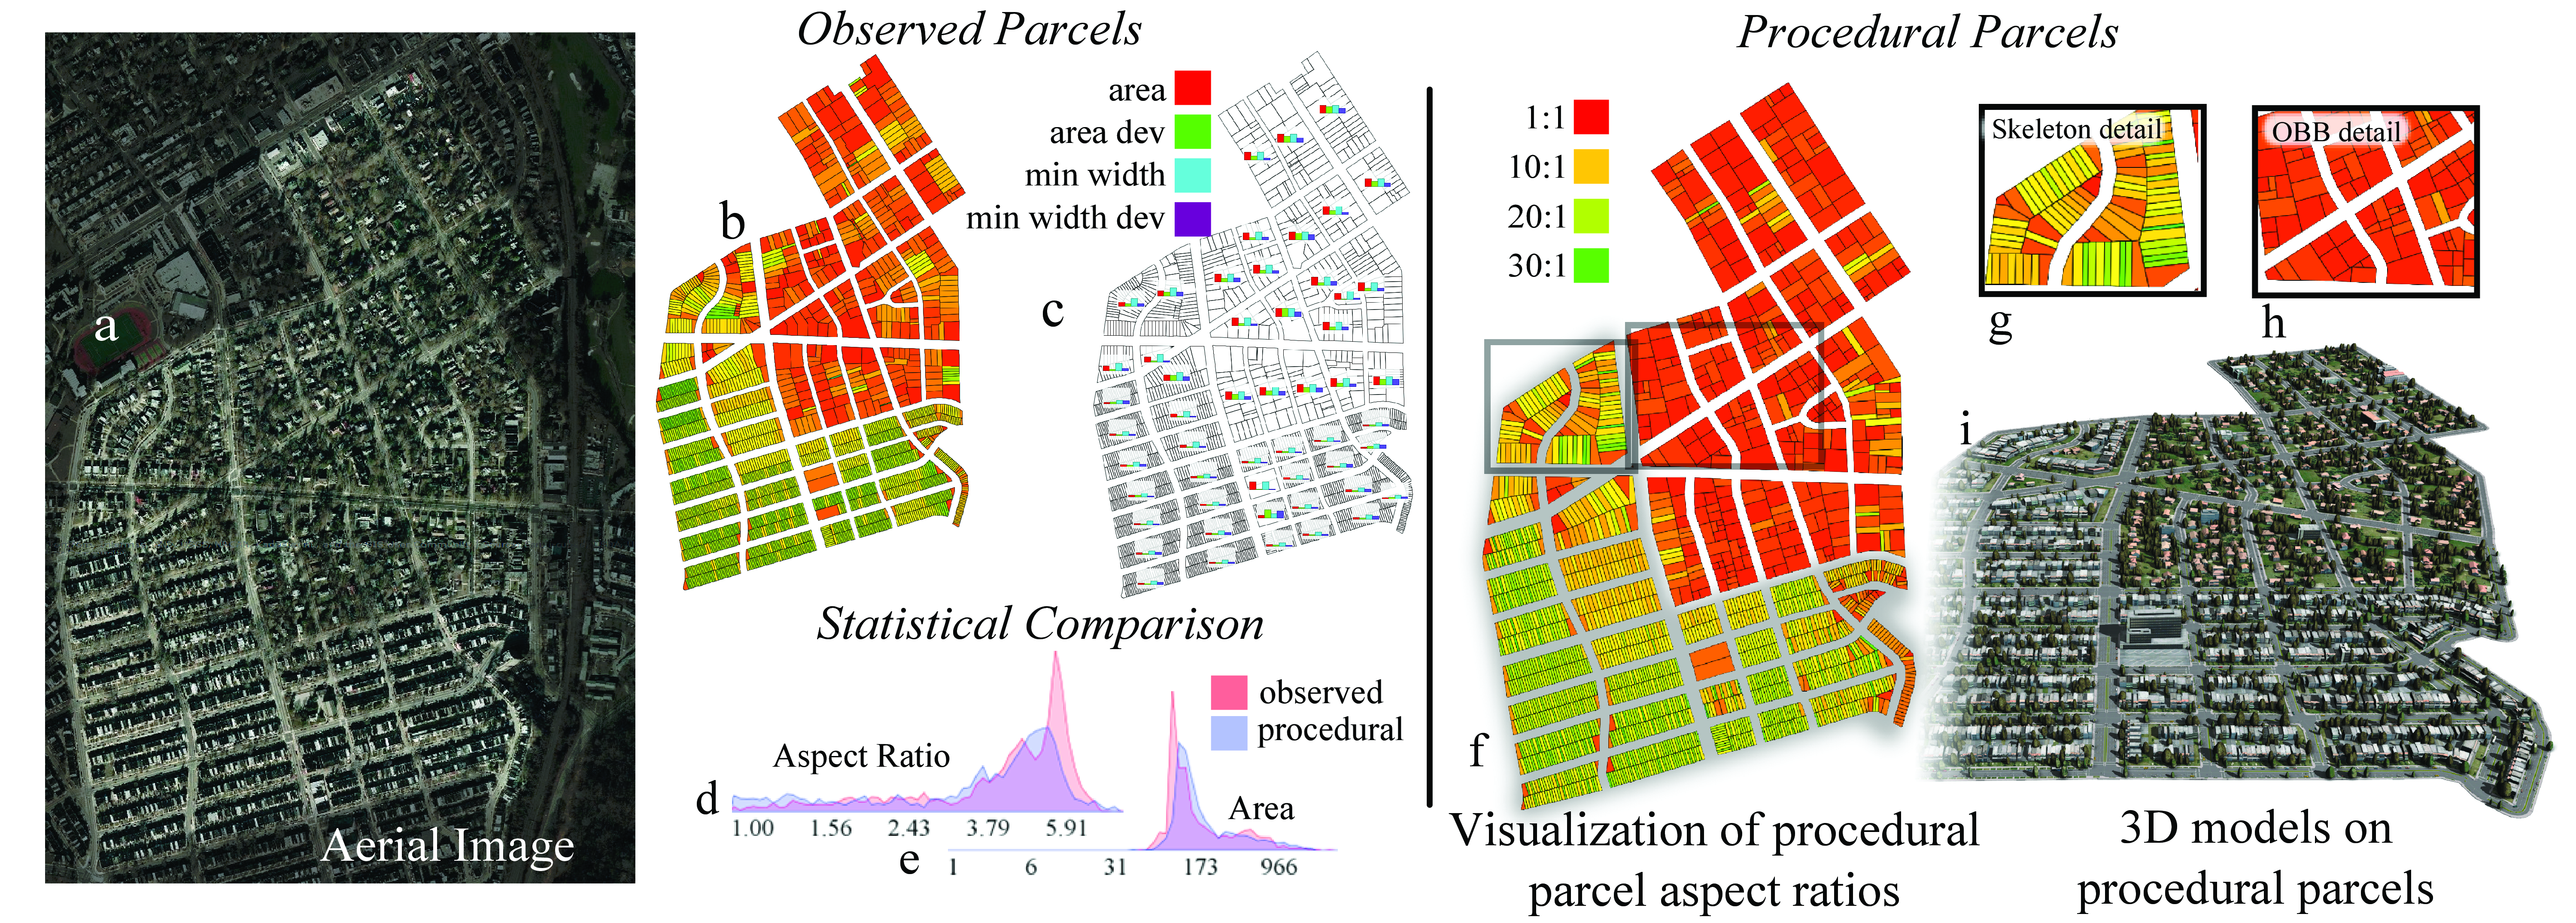
\includegraphics[width=1.0\linewidth]{figTeaser.png}

  \caption{
\label{fig:teaser}
   Procedural Parcel Generation. Our method creates parcels inside city blocks (f,i) using two different subdivision
   techniques --- \emph{skeleton} (g, shaded part of f) or \emph{OBB} (h, unshaded part of f).
   The subdivision attributes are automatically extracted from observed real-world cities (a,b,c) or determined by the user. The resulting parcel configurations
   closely resemble real-world subdivisions, as shown by our statistical and visual comparison of procedural and observed parcel data sets (d,e).
  A comparison to ~\cite{Weber09} is presented in Appendix \ref{sec:comparisonInputOutput}.
  }
\end{figure}
\end{comment}
 %%%%%%%%%%%%%%%%%%%%%%%%%%%%%%%%%%%%%%%%%%%%%%%%%%%%%%%%%%%%%%%%%%%%%%%%%%%%%%%%%%%%%%%


This chapter introduces a method for the procedural generation of city parcels from city blocks. Within an interactive procedural modeling environment the method reproduces parcel subdivisions in a distinct style, given a small number of user specified parameters and no additional user programming. The work was motivated by the real world need of a commercial procedural modeling system, CityEngine\cite{cityEngine}, a procedural cityscape generator. A fast, robust and realistic block subdivision scheme was required for the product. Given the interesting properties that we observed in the straight skeleton in previous Chapter 3, it seemed a natural choice to solve some of the geometric problems that block subdivision presented. 

To create a virtual cityscape a classical ``waterfall'' urban PGM pipeline utilises discrete stages to first create course features, which specify the inputs to finer elements. A typical pipeline features main roads, between which quarters are divided further by minor roads. Between these small roads, city blocks lie. These are subdivided individual lots, lots into footprints and from footprints, buildings . An overview of these stages is given in Fig.~\ref{fig:umPipeline}. In this chapter we address one aspect of this pipeline --- the critical problem of creating realistic city lots from blocks within an interactive PGM system. 


Here we introduce a novel method of block subdivision. We utilise the geometric self sensitivity of the straight skeleton to generate \emph{Modernist} style parcel subdivisions. 
We also present a recursive-split approach to create traditional parcel subdivisions, which is presented here in order to provide a state of the art implementation of a subdivision scheme for comparison. 
The complete system is able to retain parcel identity under interactive user edits such as moving a street intersection, and is robust enough for integration into a commercial procedural modeling tool. We conclude the chapter by comparing the results of these subdivision techniques against real-world examples.
\kawt


One of the challenges in procedurally generating parcels is creating geometry that is adaptive to the block shape. In particular identifying the centrelines of rows of parcels within irregular blocks is essential to many observed block subdivisions. We found that the straight skeleton provided a very powerful and stable centreline detection mechanism, that was well suited to interactive modeling.

%%We present a method for interactive procedural generation of parcels within the urban modeling pipeline. Our approach performs a partitioning of the interior of city blocks using user-specified subdivision attributes and style parameters. Moreover, our method is both robust and persistent in the sense of being able to map individual parcels from before an edit operation to after an edit operation - this enables transferring most, if not all, customizations despite small to large-scale interactive editing operations. The guidelines guarantee that the resulting subdivisions are functionally and geometrically plausible for subsequent building modeling and construction. Our results include visual and statistical comparisons that demonstrate how the parcel configurations created by our method can closely resemble those found in real-world cities of a large variety of styles. By directly addressing the block subdivision problem, we intend to increase the editability and realism of the urban modeling pipeline and to become a standard in parcel generation for future urban modeling methods.

%-------------------------------------------------------------------------
% INTRODUCTION
%-------------------------------------------------------------------------
\section{Introduction}
\label{sec:parcelIntroduction}

The urban procedural modeling pipeline has been widely applied to several fields including virtual environments, urban reconstruction and architecture.
%For example the commercial system CityEngine\cite{cityEngine} has been used for special effects in movies such as \emph{Cars 2} (2011) \emph{Total Recall} (2012), as well as architectural purposes such as planning the Swiss Village within Masdar city. 
While there have been numerous systems for the generation of street networks\cite{Chen08}, buildings\cite{Pascal06} and facades\cite{Mueller:2007:IBP}, there has been relatively little attention paid to the generation of parcels from city blocks. Those systems which do exist are either not responsive to the block geometry, unrealistic, or are not easily controlled. Increasing the fidelity and speed of parcel subdivision benefits the quality and speed of the entire urban modeling pipeline.

%%Interactive large-scale urban modeling is becoming increasingly popular in computer graphics research and in applications to several fields including gaming, urban planning, and navigation tools. A key reason for the popularity of interactive urban modeling is the ability to quickly create large complex models. The major steps of a typical modeling task include (i) creating the underlying terrain and general land-use pattern of the city or urban area, (ii) generating an interconnected road network, (iii) subdividing the space in between roads (i.e., blocks) into parcels, and (iv) populating parcels with buildings, parks, and other urban structures. In this paper, we focus on the third major step in this pipeline: providing a comprehensive and fully interactive approach for subdividing blocks into parcels, a task which has been largely ignored in previous computer graphics systems potentially resulting in unrealistic and implausible results.

Our high-level approach was to emulate two distinct modes of block subdivision from the urban planning literature. Carmona\cite{carmona2003:PP} identifies two such modes:

\begin{itemize}
\item \emph{Modernist} patterns position ``buildings as separate pavilions freestanding in a more generalised type'', examples are given in Fig.~\ref{fig:parcelTypes}, left. This design often appears ``in its pure form when built on greenfield sites'', and is generally used in lower density neighbourhoods that are homogeneously planned. The parcels will typically be rectangular, have street access at the front, and neighbour other blocks at the sides.
\item \emph{Traditional} patterns of subdivision are characterised by a ``generalised highly connected mass'' and ``\emph{streets and squares} and a small-scale, finely meshed street grid''. As demonstrated in Fig.~\ref{fig:parcelTypes}, right, this design is prevalent in historic cities and unplanned high density areas. The parcels may or may not have street access, with small lanes and courtyards offering access to occupants. Often traditional subdivision patterns emerge in an ad hoc manner, rather than the block being designed, as is common with Modernist patterns. 
\end{itemize}

\begin{figure}
\centering
\def\svgwidth{1.\columnwidth}
\includesvg{14-parcels/images/parcelTypes}
\caption[Two parcel types]{\label{fig:parcelTypes} Clockwise from top left: Glasgow, Shanghai, Param, and Nevada (\copyright Google Maps). Left: Modernist parcel subdivisions. Right: Traditional parcel subdivisions.}
\end{figure}


We present an algorithm to model the modernist pattern, and refer the reader to \cite{twak12} for the details of the traditional subdivision algorithm. As Carmona notes there is something of a continuum between these two ideals -- ``Indeed, it is not clear at what point \emph{space between buildings} becomes \emph{open space containing buildings}''. Both designs are often observed with a uniform structure with rectangular, quadrilateral or sometimes polygonal shape\cite{curdes1997stadtstruktur}.
\kawt

After discussing the several parcel subdivision schemes in the corpus in the following Sec.~\ref{sec:parcelPrevious}, we will detail the inputs and outputs to our two subdivision systems in Sec.~\ref{sec:blockSubdivision}. The Modernist subdivision style forms the basis for the \emph{skeleton} subdivision algorithm, detailed in Sec.~\ref{sec:skeletonSubivision}, while the traditional style is approximated by the \emph{oriented bounding box} (\emph{OBB}) algorithm of \cite{twak12}.
Concluding, the application of these techniques to real-world block patterns is presented and evaluated in Sec.~\ref{ref:results}.

%% Moreover, parcels usually have a rather regular or uniform structure that is typically a deep rectangle, wide rectangle, approximate square, quadrilateral, or sometimes polygonal \cite{curdes1997stadtstruktur}. We seek to automate the subdivision of arbitrary block shapes, ensure the aforementioned set of urban characteristics are met, and provide user-controlled realistic parcels that approximate the forms used in practice. This level of automation gives more time to designers to concentrate on high-level design decisions, including during virtual world content creation. 

%% Our approach for parcel generation uses a combination of two subdivision methods to reproduce the aforementioned two parcel varieties, including mixed-types, and to ensure a set of subdivision attributes are satisfied. 

%-------------------------------------------------------------------------
% PREVIOUS WORK
%-------------------------------------------------------------------------
\section{Existing Parcel Subdivision Techniques}
\label{sec:parcelPrevious}

The existing literature addressing procedural parcel subdivision comes mostly from computer graphics. Given a city block as a polygon, the task is to subdivide it into a number of non-overlapping parcel-polygons, giving the user control via a number of parameters.

Fig.~\ref{fig:weregreat} gives several examples of existing automated parcel subdivision techniques. The first approach that the authors are aware of, from within computer graphics, by Parish and M\"{u}ller\cite{Parish:2001:PMC} (Fig.~\ref{fig:weregreat}, brown), has gained the most traction and variations. The parcel is recursively split into two using straight lines (top, with darker splits created before lighter ones). The variations include different criteria for selecting the line to split a region and the termination criteria, although the literature often gives trivial treatment to the details ---
\begin{itemize}
\item Parish chooses to split perpendicular to the longest pair of edges that are approximately parallel, until the resulting parcels are below a specified area.
\item Weber\cite{Weber09} et al. assume mostly rectilinear parcels and select the longest edge adjacent to a street, before splitting perpendicular to this edge at a randomly displaced midpoint. If the resulting parcels do not have an undesired aspect ratio, they are accepted, otherwise another randomly displaced midpoint is attempted. Once the parcels are below a user specified area the process terminates.
\item Vanegas et al.\cite{Vanegas09:IDU} use the population count and number of jobs to estimate the area in their subdivision scheme at which recursion halts.
\end{itemize}

\begin{figure}
\centering
\def\svgwidth{1.\columnwidth}
\includesvg{14-parcels/images/weregreat}
\caption[Previous parcel generation approaches]{\label{fig:weregreat}Comparison of the skeleton subdivision approach to existing approaches. From left to right, the input, the parcel subdivision techniques from \cite{Parish:2001:PMC,twak06,Aliaga08,Wickramasuriya11} and our result which gives realistic result of Modernist parcel subdivision on concave blocks.}
\end{figure}

Another early approach was to use area division based on a number of sites. The \emph{Voronoi}\cite{Voronoi} diagram of a set of sites is a geometrical construct that associates every point on the plane with the nearest site. The area spanned by points associated with a single site is known as a \emph{cell}. These Vornoi cells have been used to generate street networks from a set of sites sampled by population density\cite{Sun2002}, as well as being used to specify parcel boundaries\cite{twak06} (Fig.~\ref{fig:weregreat}, yellow). Because the cells boundaries are rarely rectangular, the results are not characteristic of observed parcel subdivisions.

An alternative application of the Vornoi concept is given by Aliaga et al.\cite{Aliaga08} (Fig.~\ref{fig:weregreat}, green). He observes that blocks often have a centreline dividing two strips of parcels on either side leads. This line is approximated by the fitting of an \emph{oriented bounding box} (OBB), minimising the space between the box (a rectangle) and the block, and using the centreline of the box. Voronoi sites are then positioned on either side of this line and the cells become the parcels. The assumption of a straight line as a centreline fails for concave blocks, as in Fig.~\ref{fig:weregreat}, and still suffers from non-rectangular blocks in some situations.

In general the urban modeling community has performed block subdivision manually according to desired patterns\cite{thadani2010language, parolek2008form}. Those systems that have been created are very limited in their realism and available styles\cite{walker2011planners,halatschEtAl:2008,marshal:CDE:09}. One such example, \cite{Wickramasuriya11}, again fits an OBB to the block and generates a centreline. As shown in Fig.~\ref{fig:weregreat}, blue, these strips are then divided to approximate a certain parcel width, specified by a user-defined parameter, and clipped to the block's perimeter.  The system also generates additional access roads, a property that we do not wish to emulate since this is an earlier stage of the urban procedural modeling pipeline. This system again fails on concave parcels, and is inflexible to the local geometry of the parcel boundary. The remainder of the work from the urban modeling community has focused on parcel subdivision of coarse raster-grid environments\cite{Ko06,Alexandridis07,Morgan09}, which are not detailed enough to use for visualisation purposes.

If we wish to interactively edit a city we are faced with the further problem of retaining consistency under edits. We wish that changes to the road network, when edited interactively, only minimally affect the associated parcels created. When the changes to the shape of a block are small Lipp\cite{Lipp11} utilises mesh-warping techniques to deform the existing parcel subdivision to the new geometry while keeping the topology intact. We are not aware of any techniques in the literature that allow for larger scale interactive editing. The problem of retaining the identity of individual parcels between user edits is also unaddressed.

We find the existing work somewhat limited in the lack of interactive features and ability to deal with planned Modernist parcel subdivisions over concave parcels. We continue by introducing our solutions to these issues.

\subsection{Evaluating Parcel Subdivisions}
\label{sec:evalParcels}


Due to both the nature of procedural modeling and its relatively new appearance in the computer graphics world, evaluating any results is often difficult. Typical evaluation techniques are to show the results of the procedural system alongside real world data, such as photographs and plans\cite{Mueller:2007:IBP, Stiny:1980:gop, Chen:2008:IPS}, or to perform subjective studies to explore whether the results of a system correlate to a non-procedural workflow or user intuition\cite{Lipp08, Yu11, Merrell11}. The objective evaluation of procedural content has yet to be addressed in a detailed and consistent way.

Currently a new procedural systems are introduced with a high frequency in very different domains. Therefore there has been little requirement to compare systems within the same domain. In addition, attempting to evaluate content that ideally has the property of being ``characteristically similar'' to some example, and yet still ``varied and unique'' is a challenging and somewhat contradictory goal. Evaluating where any given system lies in relation to these two extrema is an interesting problem that has not yet been addressed. 

Our literature survey failed to identify any evaluation system for procedurally generated block subdivision. Due to the lack of existing material that evaluates procedural content in general, and procedural parcel subdivisions in particular, we introduce three per-lot metrics that we will use to evaluate our block subdivisions. These metrics were chosen because of their:

\begin{itemize}
\item{Objectivity --- the statistics are not subject to opinion.}
\item{Ease of computation --- because the test data sets are large, each of the heuristics must be fast enough to compute for every lot in a city.}
\item{Clarity --- the metrics are all sufficiently simple to implemented quickly by future researchers on the subject.} 
\end{itemize}

Therefore the per-lot metrics we have chosen are:
\begin{itemize}
\item{Area --- measured in $m^2$.}
\item{Aspect ratio --- given the smallest bounding box that encloses each lot, this is the ratio of the longest to shortest side.}
\item{Neighbour count --- the number of unique lots that the lot shares an edge with. Lots adjacent only at verticies are not counted.} 
\end{itemize}
\kawt



%\cite{Sun2002}Voroni for streets, sampled by density. \cite{twak06} Voronoi subdivision. Used for blocks 
%\cite{Aliaga08} Main axis of the OBB is calculated and sampled with points. Voronoi diagram is calculate.Taken from average parcel area. All must have road access. Each block dividied into two rows of parcels. Notes that medial axis is approximated using an OBB, since most blocks are rectnagular.
%\cite{Parish:2001:PMC} Assume convex, rectangular blocks. Divides the longest ednges that are approximately parallel until the lots are under a certain area. (Single paragraph explanation). 
%\cite{Weber09} recursive technique similar to \cite{Parish:2001:PMC}. Dominated by rectulangular parcels, boundary orthogonal to streets. Recursvly split  1) simplify all collinear edges, 2) select longest side on a street, find a point on longest side stochastically, if the ratio is below min ratio, then it is good, try several times. else pick another side that isn't longest or on street.
%\cite{Vanegas09:IDU} Function of the longest axis of the oriented bounding box of the block, and density count as inputs. Uses ~\cite{Paris:2001:PMC} or ~\cite{Aliaga08} for algorithms.
%\cite{Lipp11} smooth transform - warps the parcels to fit locally, relative to local coordinates. Local regeneration uses method from \cite{Weber09}.

%\cite{thadani2010language}
%\cite{parolek2008form}
%\cite{walker2011planners} cant' find
%\cite{halatschEtAl:2008} not relevant
%\cite{marshal:CDE:09} book, not available

% not usesd The subdivision of blocks and generation of parcels has been partially addressed in previous works. Within computer graphics research, Parish and M\"{u}ller \cite{Parish:2001:PMC} pioneered a procedural approach to urban modeling and many derivative works have since been created. Vanegas et al. \cite{Vanegas10:MAB} provides a recent state-of-the-art report of related urban modeling methods. While previous automatic block subdivision methods take into account providing egress (i.e., ensuring a parcel has street access), the methods do not always produce plausible parcel shapes, sometimes only support simple block shapes, and can yield areas within a block that are not assigned to any parcel. Within urban design and planning research, the focus of parcel generation methods has been on satisfying the major interests of real-estate investors and complying with zoning and building law regulations \cite{panerai2004urban}. While automatic subdivision is well exploited in computer graphics, in urban design blocks are partitioned according to desired patterns (e.g., \cite{thadani2010language, parolek2008form}) but the labor is often performed manually, a task which does not scale well to large urban modeling applications. Moreover, in either graphics or urban design, altering an existing city's geometry can cause unexpected changes in a block's subdivision, leading to difficult shape control and editing. Further, this challenge is only exacerbated during interactive editing. For example, a small change to road geometry can cause the subdivision for an entire neighborhood of parcels to be unwillingly altered both in number and in shape -- this lack of parcel persistence can cause the loss of prior customizations.

%We provide a brief review of previous and related work for generating the 2D and 3D geometry of urban spaces. Parish and M\"{u}ller \cite{Parish:2001:PMC} introduced an initial approach in which L-systems were adapted to resemble the growth of streets. Subsequent block subdivision was implemented as an algorithm that recursively divides the longest pair of approximately parallel edges until parcel sizes are under a user-specified threshold area. Parcels with no street access are discarded. This simple algorithm does not necessarily produce realistically shaped parcels and leaves odd-shaped empty areas inside city blocks that do not belong to any parcel.  Vanegas et al. \cite{Vanegas09:VOS} describe a block subdivision algorithm which assumes parcels are mostly rectangular. Their method computes the oriented bounding box of the parcel and uses the middle (long) axis to optionally divide the block into two areas, which are then partitioned into the same number of parcels. While all parcels will have egress, other subdivision styles are not supported, nor is parcel persistence addressed.

%More recently, Lipp et al. \cite{Lipp11} proposed a method that enables editing an urban layout. While their approach is interactive and does support a type of editing persistence, it does not focus on block subdivision. They assume the subdivision is present in the initial layout and use very simple heuristics to subdivide small blocks that may appear during an editing process (e.g., around the fringes of a street or neighborhood that is moved or transformed interactively). Several works have integrated urban simulation engines into the urban modeling pipeline.  For example, Weber et al. \cite{Weber09} describe a geometrical simulation of a growth of a city of overtime. Vanegas et al. \cite{Vanegas09:IDU} integrate an urban behavioral simulator with procedural modeling.  Neither paper innovates block subdivision -- rather they re-implement the methods in \cite{Parish:2001:PMC,Aliaga08} or \cite{Vanegas09:VOS}.  In urban design and planning, automatic methods are rarely used. The few available solutions  (e.g., \cite{walker2011planners,halatschEtAl:2008,marshal:CDE:09,Wickramasuriya11}) do not go beyond basic implementations and have very limited stylistic control (Figure \ref{fig:weregreat}).

%%Later work has built upon Parish and M\"{u}ller's paper and further developed different components. Several papers have focused on providing realistic building content (e.g., \cite{Wonka:2003:IA,Mueller:2006:SG,Lipp:2008:IEV}). Other works have concentrated on road networks. For example, Chen et al. \cite{Chen:2008:IPS} use hyper-streamlines and tensor fields to generate a road network but do not provide a novel automatic block subdivision algorithm. Galin et al. \cite{Galin10} provide a methodology to generate realistic roads between a source and destination but do not address parcel generation. 

%In contrast to previous work, we propose a guided space-partitioning based scheme. Since we perform a space-partitioning, we avoid the presence of unassigned areas. The automatic processing of our method, which seeks to satisfy a set of subdivision attributes, supports a range of block subdivision styles, and produces regular and nicely-shaped parcels despite partitioning arbitrarily shaped blocks (i.e., not only nearly rectangular blocks). Finally, our solution is designed to support parcel persistence and fast interactive editing for both local and city scale operations. 



%-------------------------------------------------------------------------
% SYSTEM OVERVIEW
%-------------------------------------------------------------------------
\section{Block Subdivision}
\label{sec:blockSubdivision}
%\label{sec:overview}

This section introduces the technical background to our parcel subdivision schemes. We first detail the data structures used for the input and output of the system, and the requirements of the output. We continue to discuss both the skeleton and OBB based subdivision algorithms.


% goal: subdivision for commercial system
% data structure, place in interactive system, 
%kill this!

%%not really used: The input to our method is a set of interconnected roads where an ordered sequence (loop) of road segments defines a block to be subdivided into parcels (Section ). Any block can have potentially one or both prototypical parcel varieties. The overall regularity and shape of all parcels is controlled by user-specified subdivision attributes that ensure:  (i) the parcels collectively partition the block (i.e., there should be no unused/unassigned space),  (ii) all parcels have the option of street access (i.e., egress),  (iii) parcels have a simple exterior boundary, often nearly rectangular, and the parcel's size and aspect ratio is controllable, and  (iv) parcels are aligned as best as possible with the adjacent street segment, if any (Section \ref{sec:blockSubdivision}).  Further, our solution includes a robust mechanism to map individual parcels from before an interactive edit operation to after the edit operation --- this enables transferring most, if not all, customizations, despite there being significant changes to the underlying road network and block geometry (Section \ref{sec:parcelConsistency}). Our framework also supports the generation of urban models of up to half a million parcels of arbitrary shapes. As shown in our results (Section \ref{ref:results}), the styles afforded by our method combined with our expressive set of attributes allow for a large variety in the subdivision results and support the generation of many subdivision styles found in real world urban layouts.

%%In this section, we provide an overview of our interactive editing system and underlying data structure. In particular, we explain our graph-based road network data structure and our procedure for the extraction and updating of blocks from a given road graph. To support (live) interactive editing of road and block attributes, we also demonstrate how to trigger updates to block subdivisions. Note that we do not explicitly discuss how to compute road geometry nor building geometry, since this is not the objective of our work.


%% A city, or fragment of a city, is represented by road network graph and its dual containing all city blocks. The road network is a planar graph $(V,E)$ with nodes $V$ and edges $E$. Each node $n\in V$ is defined by its position in $\mathbb{R}^2$ and logically corresponds to a road intersection point. Each edge $e\in E$ stores the indexes of its source and target nodes and logically corresponds to a road segment. In our implementation, the edge also stores the width of the street that it represents, and an interpolation type that determines whether the edge is a straight line segment or a curve. In the latter case, the adjacent nodes are interpolated using Bezier splines.

%A city block $B$ corresponds to exactly one face of the road network graph. City blocks are connected by a shared road segment. Thus the set of city blocks form the dual of the road network graph. This dual graph can be stored explicitly or recomputed each time it is needed from the road graph (as is the case in our system - see Section \ref{subsec:liveInteractiveEditing}). Each city block $B$ stores several attributes that determine how the block is subdivided into parcels, including subdivision style, parcel area and width bounds and split irregularity - see Section \ref{sec:algoOverview}. Some of these parameters are common to groups of blocks, while others are specific to individual blocks. 

%As with most urban modeling systems, our implementation supports editing the road geometry and block parameters, either for individual roads/blocks or for large areas of the city. The editing system determines that the contour geometry of the blocks needs to be updated (i) after road graph topology changes and/or (ii) after any road/block attribute changes. If a topology change occurs (e.g., addition or removal of a road segment), the set of blocks is updated through a planar face traversal method that efficiently extracts the cycles of the graph. For every new block the contour geometry is computed. If an attribute change occurs (e.g. a node translation or a street width change), the set of affected blocks is computed and the contour geometry of the respective blocks is updated. Block subdivision (Section \ref{sec:blockSubdivision}) is triggered for a given block $B$ whenever there is a change in either the geometry of the contour $C(B)$ of the block; or in the values of the subdivision attributes for the block. The parameters for individual blocks are mapped to the corresponding set of blocks as determined by our parcel consistency method (Section \ref{sec:parcelConsistency}).


%----------------------------------------------
\subsection{Inputs, Outputs and Goals}
\label{sec:parcelIOandGoals}

The input to the system is a set of city blocks, generated by the previous stage in the urban modeling pipeline, while the output is a set of parcel polygons, suitable for the next stage of the pipeline, creating mass models.
Our system is able to fulfil these conditions, while delivering statistically similar subdivisions over concave city blocks, controlled interactively by a few parameters. 
%We demonstrate that many of these parameters can be automatically extracted from real world data.  

The previous stage of the urban procedural modeling pipeline delivers a street-network, in our case a planar graph, $(V,E)$, of verticies, $V$, and edges, $E$. These verticies lie in the same plane in $\mathbb{R}^2$, at the road intersections. The roads represented by the edges in $E$, posses a width, and may be straight or curved. We expect that the graph is planar, and no two roads intersect, giving a 1:1 mapping between the faces of $(V,E)$ and the set of blocks. The topology of city blocks is therefore formed by the faces of $(V,E)$; unbounded faces are not considered at this time. 

Taking the geometry of a street (street width, sidewalks, intersections) surrounding the block, $B$, the street modeling subsystem creates a simple polygon describing the border of the block, $C(B)$. The polygonal border approximates curving streets and any features of the street geometry, such as pavements. This boundary is formed of $m$ verticies $C(B)= \left\{ b_1,b_2, \ldots ,b_m \right\}$ in a counter-clockwise direction. Note that such street modeling is a previous stage in the urban modeling pipeline, and like the following stage of mass-model generation is not addressed here. Every edge in the boundary is associated with a street in $E$, and a set of parameters. In our implementation we recompute the faces, blocks, and parcels as the street network is edited, or the block parameters adjusted. 

The city block, $B$, is associated with various parameters. Each of these may be specified by the user or extracted from example block subdivisions. The parameters include:
\begin{itemize}
\item the algorithm to subdivide the block into parcels, either \emph{skeleton} or \emph{OBB}
\item parcel area bounds, $( A_{min},A_{max})$: The upper and lower bounds on the area of the resulting parcels. %For all $l_i$, $A_{min} < A(l_i) < A_{max}$.
\item minimum parcel width, $(W_{min},W_{max})$: The upper and lower bounds on the length of the sides of the oriented bounding box of a parcel.
\item split irregularity, $\omega$: The deviation of a split edge from its default position, normalised in $\left[ 0,1 \right]$.
Larger values result in the split being further away from the mid-point and a larger variety of parcel areas.
\item various algorithm subdivision specific parameters. 
\end{itemize}

The output of the system is a set of polygons describing the new parcels. For every $B$ a set of $n$ parcels, $L= \left\{ l_1,l_2,\ldots ,l_n \right\}$, are created that exactly cover $B$ with no overlap; that is $\bigcup_{i=1}^n l_i =B$ and $\forall_{l_i,l_j \in L} ( l_i \cap l_j = \emptyset )$. Every parcel, $l$, is a simple planar polygon. 

%%The algorithms are controlled by high-level user-specified stylistic control parameters and also support mixed-type configurations. In all cases, the partitioning process is performed independently for each block. 

Modern procedural urban modeling systems make use of non-flat terrain and roads. In this situation, we vertically project the blocks onto the plane before subdivision and re-project the output parcels onto the terrain after. We assume that the terrain is a height field and thus sufficiently flat to preserve the planar and covering properties of the blocks and parcels.

%-------------------------------------------------------------------------
% BLOCK SUBDIVISION
%-------------------------------------------------------------------------
%\section{Block Subdivision}

To replicate the two patterns suggested by urban design work (Sec. \ref{sec:parcelIntroduction}) we introduce two independent algorithms to transform each $B$ to a $L$. Our implementation was in the Java language, within the procedural modeling system provided by CityEngine\cite{cityEngine}.

The straight skeleton (``SS'' or ``skeleton'') algorithm produces procedural Modernist subdivisions, and is introduced in Sec. \ref{sec:skeletonSubivision}. The central assumption of the algorithm is that each parcel has a similar street-frontage. The distance that each parcel occupies behind this frontage is the \emph{parcel depth}. If the depth is shallow, the block becomes a \emph{perimeter block}, with a semi-private \emph{patio} area in the centre of the block. An example of such a block is given at the top left of Fig.~\ref{fig:parcelTypes}. If the depth is high, there is no patio area, but instead often observe a \emph{centreline} in the subdivision, with a row of parcels on either side. An example of this is shown in the bottom left of Fig.~\ref{fig:parcelTypes}. The skeleton parcel algorithm uses either a partial or complete application of the straight skeleton to model perimeter and centreline blocks respectively. Typically the result of this algorithm is rectangular blocks on rectilinear street patterns, and ``wedge'' shaped blocks on curved streets.

\begin{comment}
The OBB algorithm is detailed in Sec.\ref{sec:obbSubdivision}, and creates a block subdivision in the traditional style. An adaptive recursive partitioning of the block is used, as introduced by Parish and M\"{u}ller\cite{Parish:2001:PMC}. Because of this street access is not guaranteed, but controlled by the user via a parameter. Further parameters control the distribution of width and area of the generated parcels. The parcels generated are commonly of a rectangular shape, and may exhibit greater diversity in size that those from the skeleton subdivision algorithm.

It is possible to combine both subdivision styles within one block by creating a perimeter block with the skeleton algorithm and then using the OBB algorithm to partition the central patio region.
\end{comment}

%This section presents our block subdivision algorithm by giving an overview, describing the sought after subdivision attributes, and explaining our two main subdivision algorithms.
%This section provides an overview of our block subdivision method, describes the sought after subdivision attributes, and explains our two main subdivision algorithms.

%Our approach consists of two main subdivision algorithms that enable each of the two prototypical parcel varieties inspired from urban design work (see Section \ref{sec:parcelIntroduction}).
%The subdivision scheme to model the first parcel variety is based on the straight skeleton \cite{Aichholzer95} of $C(B)$.
%Straight skeleton based subdivision enables three desirable properties that collectively yield parcels resembling the first parcel variety:
%The straight skeleton of a polygonal block ensures the following design requirements: (i) the resulting regions always have street access, which is one of the main constraints for this parcel variety; and (ii) the rear side of the generated parcels is always abutting another parcel -- a characteristic of this parcel variety. The rear-side neighbor parcels can be either parcels with street access themselves, or a central \emph{patio} parcel with no street access. The latter case is known as \emph{perimeter block} (Figure \ref{fig:strip_skeleton} right), which according to urban planners is an optimal design pattern to achieve very high urban densities without high-rise buildings. Intuitively, such a perimeter layout can be obtained by creating parcels ``around'' the medial axis of the block contour, and we exploit the fact that the straight skeleton is a linear approximation of the medial axis.

%(ii) the rear side of the generated parcels is always abutting another parcel -- another characteristic of this parcel variety; and
%(iii) the circular layout of the regions around the straight skeleton allows for the creation of the popular perimeter blocks (i.e., city blocks built up on all sides surrounding a central space), which according to urban planners is an optimal design pattern to achieve very high urban densities without high-rise buildings.

%% The second subdivision scheme is based on a recursive splitting concept as introduced in \cite{Parish:2001:PMC} and performs an adaptive spatial partitioning of $C(B)$ using oriented bounding boxes (OBBs). The result is parcels resembling the second variety, namely the presence of parcels on the perimeter of the block with egress and parcels interior to the block presumably separated by small pathways or alleys. 

%%Hybrid uses of these two methods is also possible. For example, a large block can be subdivided using skeleton-based subdivision to yield parcels of a chosen maximum depth around the perimeter and the interior space can be optionally partitioned using OBB-based subdivision.

%-----


%%While our methods support an infinite number of subdivisions for a given block, only some such subdivisions are adequate for mimicking land subdivision in real-world cities. Hence, several constraints are considered when determining suitable subdivisions, including a fairly homogeneous area distribution among the resulting parcels, parcel areas, aspect ratios and angles that meet structure construction constraints, and access from the parcels to the road network. The set of subdivision attributes that our system enforces for all parcels is provided below.

%%The detailed pseudocode for both styles is presented in Algorithm \ref{algo:subdivSS} of Appendix \ref{sec:pseudocodes}.

%-------------------------------------------------------------------------
% SUBDIVISION STYLES
%-------------------------------------------------------------------------
\subsection{Skeleton-based Subdivision}
\label{sec:skeletonSubivision}

The straight skeleton subdivision algorithm generates Modernist parcel division. Our approach is to generate a contiguous area for a row of parcels along a street (we refer to these areas as \emph{strips}) before slicing these strips along the adjacent street into parcels. This approach ensures that every parcel has street access, and that the length of street-frontage is similar for every parcel.

We observe that both perimeter blocks and centreline blocks contained such strips, and that both can be generated by varying the depth of a block from the street. However determining borders between these strips, both parallel and orthogonal to the street, is an involved problem ---
\begin{itemize}
\item We observe that at corners of blocks near street intersections one strip will give priority to another to ensure more rectangular blocks
\item To control the style of subdivision to be centreline or perimeter, the depth of the blocks from the street must also be generated as specified.
\item A special case in our algorithm is the treatment of narrow blocks, in this situation only a single strip is generated. The narrow-block threshold parameter identifies the parcels in which this behaviour is appropriate.
\end{itemize}

Our insight into this problem came after we observed that the arcs of the partial straight skeleton included a lot of the information that we required to identify the centrelines. This lead to the solution presented here which uses a partial straight skeleton to specify the depth of the strips, but cleans up the ``diagonal edges'' generated near the corners to create more realistic rectangular strips.

\begin{figure}
\centering
\def\svgwidth{0.7\columnwidth}
\includesvg{14-parcels/images/medialIssues}
\caption[A perimeter block's depth]{\label{fig:medialIssues}Left: The medial axis (dashed lines) of a polygon (solid green lines) describes points equidistant from the boundaries of the polygon (grey circles). We note that the curved (red) arcs of the medial axis require rasterisation for use in a polygonal environment and that they generate sharp corners in the faces (shaded regions). Right: The equivalent straight skeleton contains no curved arcs, and includes arcs for reflex corners.}
\end{figure}


There were several alternatives to the unweighted skeleton for generating centrelines. One possible alternative was the medial axis. The axis would introduce curved sections into our geometry, Fig.~\ref{fig:medialIssues}, leading to awkward ``sharp'' corners in medial axis faces which would have required intensive filtering to rectify. These sharp corners in faces occur on very simple concave polygons. A further disadvantage to the medial axis was the algorithm's origin as a bitmap image filtering tool~\cite{Blum67}. Only recently have algorithms emerged that calculate geometry explicitly~\cite{Joan1999,Ramanathan2003}, however the output of these systems includes parabolic segments. Given that the typical 3D pipeline operates on polygons, parabolic sections would require rasterisation before use in the typically polygonal procedural modeling pipeline. Such rasterisation comes with involved checks for geometric consistency. Finally such medial axis algorithms do not create arcs for reflex verticies, and so are unable to ``guide'' the splitting of strips in the same manner as skeleton faces.
\kawt

A further alternative was the weighted straight skeleton. This would have enabled us to move the centreline relative to each of the edges of the block, and to create perimeter blocks with different depths on each road. The weighted straight skeleton proved problematic for two reasons; firstly there was no easy mechanism to assign such depths to each road, and second there were no known commercial weighted skeleton implementations available at the time of publication.

The skeleton subdivision uses the following parameters in addition to those in Sec.~\ref{sec:parcelIOandGoals}.
\begin{itemize}
\item The maximum parcel depth, $d_{\text{offset}}$, determining whether the centreline or perimeter styles of subdivision occur. 
\item A street priority scheme, either \emph{StreetWidth} or \emph{StreetLength}. This specifies the direction in which diagonal edges should be resolved.
\end{itemize}

%% Our choice of the straight skeleton is further supported by our observations of how urban planners often, out of intuition, draw an approximate medial axis to homogeneously subdivide blocks, especially in residential areas.

% bump pseudo code up
% add discrete list of extra parameters

%%This subdivision style creates parcels resembling the first prototypical parcel variety, i.e., parcels whose front-sides are along a street, and rear-sides are adjacent to other parcels.
% --- all lots must have street access, blocks frequently have center-lines between rows of parcels, parcel boundaries are normally straight lines, and the direction that parcels face at street intersections is complex. 

%%We made several observations which directed the design of our algorithm. The first was that every parcel should have street access, and that the direction of this street access at intersections varied. This lead us to the concept of \emph{strips} of parcels, which follow roads. Further observations were that the initial split was frequently the common centerline between rows of parcels on either side of the block, and the rear edges of the parcels were normally straight.

%%A polygonal skeleton supports these observations as it identifies both the potential strips and the centerline. We found the straight skeleton the most realistic, since other techniques, such as the medial axis, introduced curved segments. Therefore our fist subdivision method computes the initial split contour via the straight skeleton, identifying the depth of the parcels via strips. Subsequent splits cast rays from the street edges to position the sides of the parcels.


%----------------------------------------------
\subsubsection{Applying the Straight Skeleton}
\label{sec:skeletonInitial}

%To define the initial split contour, the user defines a perpendicular distance, $d_{offset}$, from the block contour, $C(B)$, to an inwards offset contour, $C'(B)$. Intuitively, this value corresponds to the maximum depth of the parcels (e.g., the distance from the road to the rear of a parcel). \minorrev The contour is calculated by a partial application of the straight skeleton to $C(B)$, (Figure \ref{fig:strip_skeleton}), via the CGAL library\cite{cgal}, i.e., the library simulates the intersection of the roof model of~\cite{Aichholzer95} with a horizontal plane at a specific height, creating the required offset contour.
%
%If the $d_{offset}$ value is sufficiently large (e.g., infinity), then the area enclosed by the initial split contour collapses. Alternatively the value for $d_{offset}$ defines an offset contour $C'(B)$ of non-zero area, forming a closed inner \emph{patio} region, with no direct access to roads. This inner region may be disconnected if the initial block is non-convex.  The patio can be further partitioned using an arbitrary subdivision style. 

To define the depth of the strips, the user defines a perpendicular distance $d_{\text{offset}}$ from the block contour $C(B)$ to an inwards offset contour $C'(B)$.
This value corresponds to the maximum depth (distance from the road to the rear) of the parcels.
If $d_{\text{offset}}$ is sufficiently large (e.g., infinity), then the area enclosed collapses and
the rear side of any resulting parcel will be directly adjacent to another parcel, leading to centrelines between rows of parcels.
Alternately, if the $d_{\text{offset}}$ value is sufficiently small, the partial skeleton application defines 
a closed inner \emph{patio} region, with no direct access to roads. This inner region may be disconnected if the initial block is concave, as in Fig.~\ref{fig:stripskeleton} right, and can be further partitioned using an arbitrary subdivision style.
While setting an infinite value for $d_{\text{offset}}$ is typical and better complies with the first parcel variety,
inner \emph{patios} are not uncommon and we designed our skeleton-based subdivision to also support them.
The contour $C'(B)$ is calculated (via the CGAL\cite{cgal} library) by a partial application of the straight skeleton to $C(B)$ to offset distance $d_{\text{offset}}$, as shown in Fig.~\ref{fig:stripskeleton}, 
by computing the intersection of the roof model of \cite{Aichholzer95} with a horizontal plane at a specific height.

\begin{figure}
\centering
\def\svgwidth{0.7\columnwidth}
\includesvg{14-parcels/images/stripskeleton}
\caption[A perimeter block's depth]{\label{fig:stripskeleton}Left: The straight skeleton of a polygon, showing $C(B)$ (black line). Right: A partial application of the straight skeleton computes the offset contour $C'(B)$ (dashed lines) at distant $d_{offset}$. Note that the contour may split the innermost, or \emph{patio}, region into several portions (a,b). The individual faces of the straight skeleton conform to our definition of a \emph{strip}, and we may take the supporting edges to be portions of the boundary of input polygon. We take these faces to be the initial set of $\alpha$-strips.}
\end{figure}


The arcs of the skeleton application specify the division of the region between $C(B)$ and $C'(B)$ into a set of strip polygons. We initially refer to these as \emph{$\alpha$-strips}, to differentiate them from the \emph{$\beta$-strips}, from which we have removed some diagonal edges. These strips are an intermediate value in our algorithm, representing a group of parcels with their primary frontage on the same logical street. Collectively they form a single connected region. 
 
Formally we define a strip, $s_i$, as a simple polygonal area within $B$, such that a single connected length of the polygon's boundary forms part of $C(B)$. These lengths are the \emph{supporting edges}, $\psi(s_i)$, of $s_i$. A block's cyclic list of $n$ strips, $LS(B) = {s_1 \ldots s_n}$, is such that it covers the area between $C(B)$ and $C'(B)$ completely and without overlap.
%, $\bigcup_{i=1}^n (s_i) = B$ and $\forall_{s_i,s_j \in LS(B)} ( s_i \cap s_j = \emptyset )$. 
The list $LS(B)$ is ordered counter clockwise, such that the last supporting edge of $s_i$ and first of $s_{i+1}$ are adjacent edges of $C(B)$. Note that we take $i+1$ to mean $(i+1) \bmod n$ in the context of a cyclic list data structure.

We initialise $LS(B)$ from the faces of the straight skeleton used to compute $C'(B)$. We observe that these faces fulfil the strip properties --- bounded by the arcs of the skeleton, and supported by an edge of $C(B)$. Any strip in $LS(B)$ may be combined with either of its neighbours and the union retains the strip properties; therefore we may union adjacent faces in $LS(B)$ according to whether they lie on the same logical street, $e \in E$ in our street graph. In this manner we create a single $\alpha$-strip for every logical street, as in Fig.~\ref{fig:take_corner}, b.

\subsubsection{Removing Diagonal Edges}


The $\alpha$-strips computed from the skeleton faces suffer from diagonal edges at the intersection of logical streets as shown in Fig.~\ref{fig:take_corner}, b. As illustrated in Figure~\ref{fig:take_corner} c-g, we correct these edges, by modifying $LS(B)$ to transfer a near-triangular region from the strip on one side of an offending edge to the strip on the other side. We refer to these corrected strips as $\beta$-strips.


\begin{figure}
\centering
\def\svgwidth{0.8\columnwidth}
\includesvg{14-parcels/images/takecorner}
\caption[Strips sharing a block's corner]{\label{fig:take_corner}The $\alpha$-strips (solid colours, b) are recovered from the skeleton (a) and logical streets (bold lines, b). This leaves undesirable diagonal edges, such as that between the brown and green $alpha$-strips. Given the classification $T(v_i) \in$  \emph{None}, \emph{Previous} ($P$) or \emph{Next} ($N$), we reassign regions (shaded, c), to create the set of $\beta$-strips. In the example (c-e) we use the classification scheme $StreetLength$, specifying the direction \emph{Previous}. The subsequent splits are computed over these $\beta$-strips (f).}
\end{figure}

Let the shared supporting vertex between each pair of $\alpha$-strips $s_i$ and $s_{i+1}$, be designated $v_i$. The shared boundary of these two strips forms the diagonal edges we are concerned with, one end of which is $v_i$. We provide a classification $T(v_i) \in \left\{\text{\emph{Previous, Next, None}}\right\}$, to specify which of the pair of strips will gain the region, and which will lose the same region. A vertex with the property \emph{Previous} (respectively \emph{Next}), will assign a region to the previous (next) strip, given the counter-clockwise vertex ordering. No action is taken with a value of $T(v_i) = $\emph{None}.


The values of $T(v_i)$ may be assigned by one of two \emph{street priority} schemes, determined by a per-block parameter specified by the user. When the angle of the supporting edges at $v_i$ is reflex we always assign $T(v_i) = $\emph{None}. For the remaining $v$, we choose between the following two schemes:
\begin{itemize}
\item \emph{StreetWidth}. If the average width of the street edges associated with the supporting edges of $s_i$ is greater (respectively lesser) than those of $s_{i+1}$ then $T(v_i) = $ \emph{Previous} (\emph{Next}).
\item \emph{StreetLength}. If the length of the supporting edges of $s_i$ is greater (respectively lesser) than those of $s_{i+1}$ then $T(v_i) = $\emph{Previous} (\emph{Next}).
\end{itemize}

We find that in most most urban environments the parcels face the most important and thus widest street; therefore we use the $StreetWidth$ scheme by default. There are situations in which this assumption is not suited. For example, residential street patterns in which parcels prefer to face the quieter, and longer, residential streets, rather than the wider and busier access-streets. In our experiments it proved difficult to make this distinction automatically, so we allow the user to assign this parameter manually.

Given the parameter $T(v_i)$, we calculate the direction in which to reassign the region, shown in Fig.~\ref{fig:take_corner}, c, creating the set of $\beta$-strips. The region is removed from strip $s_x$, where $s_x=s_{i}$ if $T(v_i) = $\emph{Next}, or $s_x=s_{i+1}$ if $T(v_i) = $\emph{Previous}.
The region is removed by cutting between two points. The \emph{primary} point is the location on the boundary of both $s_i$ and $s_{i+1}$ that is furthest, at distance $z$, from $C(B)$,  (Fig. \ref{fig:take_corner}, d). The \emph{secondary} point is located on $C(B)$ at a distance $z$ from  $v_i$ along $psi(s_x)$.
The region is then unioned to the strip $s_y$ where $s_y = s_{i+1}$ if $T(v_i) = $\emph{Next}, or $s_y = s_{i}$ if $T(v_i) =$ \emph{Previous}. Finally we recompute the skeleton arcs to remain perpendicular to the local edges in $\psi(s_y)$, (Fig.~\ref{fig:take_corner}, f), in order to ensure we are able to guide the subsequent splits in the following stage (Fig.~\ref{fig:take_corner}, g). After processing each pair of adjacent strips in $LS(B)$, we are left with the list of $\beta$-strips. 

Strips with a small supporting edge are rarely observed, and so are undesirable. If a strip loses area to both neighbouring strips, and the distance between the secondary points is small, we move the secondary points to the same location. A threshold distance of $2W_{min}$ determines whether we move both points to the point closest to their mean location on $\psi(s_y)$. This ensures that the entire strip is reassigned to its neighbours (Figure~\ref{fig:take_corner}b, cyan and brown). Such a strip is removed from LS(B). On small lots this routine may introduce ``zig-zag'' artifacts, these are resolved as in Fig.~\ref{fig:mergeissue}.

\begin{figure}
\centering
\def\svgwidth{0.8\columnwidth}
\includesvg{14-parcels/images/mergeissue}
\caption[A problem with tolerances]{\label{fig:mergeissue}The green and yellow strips take enough area from the blue and red strips to trigger their removal, as $z$ become less than $2W_{min}$ (ab). If we move the secondary point to a mean location, we may be left with ``zig-zag'' artifacts after the strip is removed (c). In this situation we average the location of the primary points (d). Given that the distance between these primary points is small, we have found that this causes very few problems.}
\end{figure}

%The motivation behind this process is to (i) extend the lot's centerline such that it reaches $C(B)$ as orthogonally as possible, and (ii) allow a parameter controlling the direction (street access) of the parcel at intersections.


%----------------------------------------------
\subsubsection{Splitting Strips into Parcels}
\label{sec:skeletonSubsequent}

To subdivide the $\beta$-strips into parcels, a set of points are sampled approximately equidistantly on $\psi(s_i)$, as shown in Fig.~\ref{fig:slice2}. Rays from these points, perpendicular to the nearest edges of $\psi(s_i)$, split the $\beta$-strip into parcels. We ``snap'' rays to nearby verticies to create cleaner geometry. The distance between the points is normally distributed around $(W_{min} + W_{max})/{2}$, with $\sigma^2 = 3\omega$, and clamped to the length of $\psi(s_i)$. This process adds a random displacement to the ray-origin points to create less uniform parcels. 
To prevent local perturbations in $\psi(s_i)$ adversely affecting the parcel geometry, we limit the rays to each skeleton face. If the ray crosses a skeleton edge, it follows the edge to the boundary of the strip, as illustrated in Fig.~\ref{fig:slice2}b. 

\begin{figure}
\centering
\def\svgwidth{0.7\columnwidth}
\includesvg{14-parcels/images/slice2}
\caption[A problem with naive strip splitting]{\label{fig:slice2}The split operation divides a $\beta$-strip's area (solid colour) into parcels with rays (dashed lines). Top: The naive approach leads to unrealistic splitting as an eccentric local normal to the supporting edge (bold lines) may propagate in an uncontrolled manner. Bottom: We constrain split-lines to the skeleton faces they are within to achieve a more realistic effect.}
\end{figure}

There are several special cases that are handled independently as post processing steps: % shallow parcels, small parcels and triangular parcels.
\begin{itemize}
\item 
There are situations in which the block is too shallow to accommodate the two rows of parcels assumed by the algorithm. In this case we group shallow parcels and replace them with parcels generated similarly to the skeleton subsequent split technique. 
%\item If a parcel is deep, the area may be unacceptably large. To mitigate this effect, blocks of area larger than $A_{max}$ are split again, via a second ray cast from the street.

\item 
Triangular parcels and parcels with small areas are repeatedly unioned with their neighbours until they are either larger than the minimum area ($A_{min}$), neither small nor triangular, or there is only one remaining parcel. We union such parcels with the adjacent parcel with which it shares the longest boundary.
\end{itemize}

As illustrated in Fig.~\ref{fig:forPerim}, the diagonal edge removal and the splitting of strips into parcels works in the same way regardless of the value of $d_{\text{offset}}$, that is whether we use a partial or a full skeleton application. 

\begin{figure}
\centering
\def\svgwidth{1.0\columnwidth}
\includesvg{14-parcels/images/forPerim}
\caption[Assignment in a perimeter subdivision]{\label{fig:forPerim}Our algorithm to compute the partial skeleton (left), remove diagonal edges (middle) and split the strips (right) demonstrated on a block with a patio region.}
\end{figure}

The pseudocode for the complete skeleton subdivision algorithm is given in Fig.~\ref{algo:subdivSS}.

\begin{algorithm}

\textit{ subdivSkeleton($B$) }
\begin{algorithmic}
\STATE $L \leftarrow \emptyset $
\STATE $SS \leftarrow \textit{ computeSkeletonOffset} (C(B), d_{\text{offset}} )$
\STATE $LS \leftarrow \emptyset $
\FOR {each face $f \in SS$}
  \STATE $\textit{ Append convertToStrip } (f) \textit{ to } LS$ 
\ENDFOR
\STATE $LS2 \leftarrow$ mergeOnLogicalStreets ($LS$) 
\STATE $LS3 \leftarrow$ \textit{ fixDiagonalEdges } (LS2)
\FOR {each strip $s$ in LS3}
  \STATE slice ($s$)
\ENDFOR \newline
\textit{ processSmallLargeOrTriangularParcels($LS$, $A_{min}$, $A_{max}$) } 
\end{algorithmic}

\line(1,0){150} \newline
\textit{ fixDiagonalEdges($LS$) }

\begin{algorithmic}
\FOR{each strip $s_i \in LS$}
  \STATE $v_i \leftarrow $ vertex between $s_i$ and $s_{i+1}$
  \STATE $t \leftarrow $ triangular portion at $v_i$
  \IF {$T(v_i) = Previous$}
    \STATE assign $t$ to $s_i$
  \ENDIF % no else if?
      \IF {$T(v_i) = Next$}
    \STATE assign $t$ to $s_{i+1}$
  \ENDIF
\ENDFOR
\FOR{each strip $s_i \in LS$}
  \IF { $\psi (s_i) < 2W_{min}$}
      \STATE remove $s_i$ from $LS$
      \STATE merge primary verticies
  \ENDIF
\ENDFOR

\end{algorithmic}
%----------------------------------------

\line(1,0){150} \newline


%----------------------------------------
% Slice routine
%----------------------------------------
\textit{ slice($s$) }
\begin{algorithmic} 
\STATE $origins \leftarrow$ sample $\psi(s)$ by $n((W_{min}+W_{max})/2, 3\omega)$ 
\STATE $remainder = \bigcap$ offset faces of $s$ % reads: &quot;union of offset faces of s&quot; - is this clear?
\FOR{each point $p \in origins$}
  \STATE $normal \leftarrow$ average normal of $B$ near $p$
  \STATE Create a ray, $r$, from $p$, in direction $normal$
  \STATE $\left[ left | right \right] \leftarrow$ slice $remainder$ by $r$
  \STATE Append $left$ to $L$
  \STATE $remaining \leftarrow right$ 
\STATE Append $remaining$ to $L$
\ENDFOR
\end{algorithmic}

\caption{
\label{algo:subdivSS}Skeleton parcel subdivision pseudocode.}
\end{algorithm}%--------------
%----------------------------------------


%===========================================

\begin{comment}
\subsection{OBB-based Subdivision\textdagger}
\label{sec:obbSubdivision}

The orientated bounding box algorithm generates parcels in the traditional style. The resulting subdivision contains mainly rectangular parcels with and without street access. The OBB based subdivision algorithm has a single additional per-block parameter, $\xi$, to specify the preference for street access.

The algorithm recursively performs a binary partitioning of the block until certain termination conditions are met, as in Fig.~\ref{fig:subdivOBB}. The partitioning is via a straight line that splits the block into two. 

%%This subdivision style creates parcels resembling the second prototypical parcel variety, i.e., quadrilateral parcels with and without street access, by using an adaptive spatial partitioning. 
To determine each split line,
the minimum-area OBB that covers the block is computed.
The pivot point of the split line is given by
the midpoint of the largest edge of the OBB, translated by a random distance proportional to $\omega$.
The direction of the split line is given by the
direction of the smallest edge of the OBB.

%Here we note that in the case of a rectangular block, both the OBB and skeleton algorithms produce similar, if rotated, centrelines. In near-rectangular situations the OBB gives a cleaner and simpler central split line than the OBB subdivision due to the geometric sensitivities.

%It is worth noting, that if the block shape is near-rectangular, the middle axis of the
%OBB is roughly equivalent to the straight skeleton but will not be curved, or overly
%affected by reflex corners in the street graph. Thus, while we could use the straight
%skeleton to generate the initial split line, using the block's OBB turns out in practice to yield a more robust mechanism.  

The process finishes when the area of a parcel is within $(A_{min},A_{max})$, or the street frontage is within $( W_{min},W_{max})$. If the split-line would create a block without street access, the orientation of the split line is rotated by $90$ degrees with probability $\xi$. This parameter controls the preference of a parcel towards street access, with higher values (closer to $1$) making it more likely that all parcels in the block will have street access.

%%For subsequent recursive splits, we also found OBB-based partitioning to yield very robust and well-behaved subdivisions. 

%At each step, each parcel is split into two smaller parcels, which are recursively split into more parcels until the area of the resulting parcels
%is within $(A_{min},A_{max})$ or the width of the front side of the parcel is within $( W_{min},W_{max})$.
%If a parcel resulting from a split has no street access, the direction of the split line is rotated $90$ degrees about the %normal vector of the
%plane containing the block, with probability $\xi$,
%where $\xi$ is a user-specified attribute in $\left[ 0,1 \right]$ that indicates the preference for parcels with street access.
%Larger values of $\xi$ result in more parcels having street access:
%If $\xi = 1$ street access is always guaranteed, while if $\xi = 0$ parcels with no street access are frequent.
%the orthogonal vector to the initial split line is used, and
%See (Algorithm \ref{algo:subdivOBB} in Appendix \ref{sec:pseudocodes}) for more details.

Our method takes into account the following additional considerations during subdivision:

\begin{itemize}

\item
edge alignment -- to increase the performance of subdivisions under interactive editing operations, we find the best-fitting OBB by fitting OBBs that align with at least one of the parcel edges,

\item
random seeds -- to increase the stability of subdivisions under interactive editing operations, the random seeds for the recursive splits of a given parcel are computed before the recursive call to the subdivision function,

\item
snap to block contour verticies -- if the split line is within a threshold distance from one of the verticies of the contour of the original block, the pivot point of the split line is set to that vertex.
\end{itemize}

%--- Figure ---
\begin{figure}
\centering
\def\svgwidth{0.6\columnwidth}
\includesvg{14-parcels/images/figSubdivOBB}
\caption[A problem with naive strip splitting]{\label{fig:subdivOBB}Oriented bounding box subdivision. This adaptive algorithm recursively splits a parcel into two smaller parcels
           along the minor axis of the oriented bounding box of the original parcel. The subdivision continues
           until user-specified shape attributes are satisfied.}
\end{figure}

%--------------

The OBB algorithm only considers local geometry, unlike the skeleton algorithm that considers the entire block. However this gives the OBB the advantage that it is locally robust against distant edits in the shape of the block. 

The complete OBB algorithm is presented in Fig.~\ref{algo:subdivOBB}.

%% unused: This recursive approach considers only the geometry of the parent shape and road access, instead of the geometry of the entire block (Figure \ref{fig:subdivOBB}). As a result, recursive OBB subdivision is very stable in the sense that localized changes in the block geometry will typically only affect the parcels nearby the parts of the geometry that are modified.
% now he;s just talking crap: Notice that the inner region subdivisions could alternatively be computed using the same \textit{slice} operation as the skeleton subdivision, since the two regions obtained upon the initial OBB split conform to our definition of a strip. While the \textit{slice} operation is suitable for the relatively thin strips generated by the initial split contours in skeleton subdivisions, applying this operation for subsequent splits in the OBB style will likely result in parcels with atypical aspect ratios. In practice, for inner regions, recursive use of OBB splits has proven to be more suitable than \textit{slice} operations for obtaining subdivisions that comply with user-specified shape parameters.

\begin{algorithm}

\textit{ subdivOBB($B$) }
\begin{algorithmic}
\STATE $L \leftarrow \emptyset$
\STATE $\textit{recSubdivOBB}(C(B))$
\end{algorithmic}

\line(1,0){150} \newline
\textit{ recSubdivOBB($l$) }


\begin{algorithmic}
%\IF {area or width attributes not satisfied}
\IF {$area(l) \notin ( A_{min},A_{max})$ \AND $frontSideWidth(l) \notin ( W_{min},W_{max})$}

  \STATE $s \leftarrow \textit{computeSplitLine} (l)$
  \STATE $ \left [ l_A, l_B \right] \leftarrow \textit{split} (B, s)$
  \IF {$l_A$ or $l_B$ have no street access}
  	\STATE Rotate $s$ $90$ degrees about the normal vector of the plane containing $B$, with probability $\xi$
  	\STATE $ \left [ l_A, l_B \right] \leftarrow \textit{split} (B, s)$
  \ENDIF
  \STATE $ \textit{recSubdivOBB} (l_A)$
  \STATE $ \textit{recSubdivOBB} (l_B)$
\ELSE
  \STATE Append $l$ to $L$
\ENDIF
\end{algorithmic}


\line(1,0){150} \newline
\textit{ computeSplitLine($l$) }
\begin{algorithmic}
  \STATE $OBB \leftarrow \textit{computeOBB}(l)$
  \STATE Let the direction of $l$ be the direction of the shortest side of $OBB$
  
  \STATE Let the pivot point of $l$ be the middle point of $OBB$  
  
  \STATE Apply a random translation of magnitude $\omega \cdot d_{OBB}$ to the pivot point of $l$, where $d_{OBB}$ is the length of the shortest side of $OBB$
\end{algorithmic}

\caption{\label{algo:subdivOBB}OBB subdivision pseudocode.}
\end{algorithm}

%-------------------------------------------------------------------------
% Parcel Consistency under Live Editing
%-------------------------------------------------------------------------

%----------------------------------------------
\section{Parcel Consistency under Live Editing\textdagger}
\label{sec:parcelConsistency}

Given an urban procedural modeling pipeline that generates a road network, blocks, parcels and mass models it is a common operation to allow users to edit the system interactively. For example users may customise:

\begin{itemize}
\item the location of verticies in the street network graph.
\item the parameters for a block's parcel subdivision.
\item the mass-model grammar associated with a particular parcel.
\end{itemize}

This raises the problem of maintaining the consistency of parcels under various editing operations --- as the user uses a mouse to move the verticies of a parcel, rotate or scale the entire parcel, how do we ensure that the structures assigned to each parcel remain consistent? Given that considerable time and effort may have gone into customising a building on a particular parcel, it is unreasonable that small editing operations would undo this work. It is therefore necessary to give predictable continuity under live editing to as greatest extent as possible. This is illustrated in Fig.~\ref{fig:consistency_intro}.

\begin{figure}
\centering
\def\svgwidth{0.7\columnwidth}
\includesvg{14-parcels/images/consistency}
\caption[The parcel matching problem]{\label{fig:consistency_intro}A street network (bottom left) may be interactively modified in several ways (a-e). We use our matching function to compute the location of each parcel, and show the location of a given parcel (blue house) after each editing operation; moving an edge (a); editing the curve of two edges(b); changing the width of a street (c); changing the subdivision style (d) or scaling the street network (e).}
\end{figure}

The parcel subdivision algorithms themselves may produce a different shape and number of parcels after such editing operations. It is inevitable that parcels must be added and removed from a block during such operations to maintain correlation with parameters, such as minimum and maximum area. Therefore, in \cite{twak12} the continuation of this work presents a solution to the \emph{parcel matching} problem, retaining the identity of a parcel throughout an editing operation. %Futhermore this solution is decoupled from the parcel algorithms in the previous section, offering instead a general solution.

% discuss editing continually with a mouse.

%This section presents the problem of consistent relative location of any given parcel within a block and discusses its relevance to live interactive editing of urban models. It also proposes a solution to the parcel consistency problem that has been implemented in our parcel generation system.
%Changes in the geometry or the topology of a road network require updating not only the road network itself (e.g., lanes, sidewalks, intersections), but also the shapes defined by the road network, specifically blocks and parcels. A system that follows the urban modeling pipeline sequentially typically proceeds by first creating the road network, then extracting the blocks as faces of a planar graph, and finally subdividing the extracted blocks into parcels (e.g., \cite{Parish:2001:PMC, Vanegas09:IDU, Weber09}). In this type of systems, when an urban model is regenerated, the connection between the entities of the previous model and the entities of the new model has little importance. In live editing, however, editing operations include large-scale modifications to the road network, small displacements of road network vertices or edges, and changes in the attributes of a subdivision. Many of these edits are sufficiently small and localized for a correspondence between the sets of parcels at two consecutive states to be expected and desired. For this reason, any urban modeling system that aims to support interactive editing of road networks, blocks and parcels, must support parcel location consistency. In spite of this requirement, existing urban modeling systems have not addressed or proposed solutions to the parcel consistency problem.

%%The consistent location of parcels under live editing operations is crucial to guarantee persistence in the relative location of specific objects in the urban models. Consider, for instance, a parcel with an associated set of parameterized rules that procedurally generates a building in the parcel. Assume that the rule parameters determine the geometry and textures of the building. If no matching between the parcels of two consecutive subdivisions of a same block was enforced, such parameters would either be lost or would be inherited at random from the parcels in the previous subdivision. By avoiding this randomness, the relative location of a building with a distinctive style is preserved.

\end{comment}

%-------------------------------------------------------------------------
%-------------------------------------------------------------------------
%-------------------------------------------------------------------------

%------------
\begin{comment}
\subsection{Parcel Matching and Inheritance\textdagger}


%%Our live editing method (section \ref{subsec:liveInteractiveEditing}) proposes a solution to the parcel consistency problem by computing a matching between the sets of the parcels of a block at two consecutive editing steps $t$ and $t+1$ (Figure \ref{fig:consistency_intro}). The pairs of matched parcels are used to establish inheritance of parcel-specific attributes. Our matching approach uses the relative position of a parcel inside its block and a metric to compute the distance between instances of a single parcel at consecutive time steps of the editing. The chosen metric is robust to changes in the vertices of the block.

As illustrated in Fig~\ref{fig:consistency_intro}, there are many possible interactive editing operations that we may perform upon our generated procedural model. We present an algorithm to deliver a matching between parcels at a time before, $t$, and after, $t+1$, an editing step.



Let $f$ be a user editing operation that modifies one or more of the following: the position of the verticies in the contour $C(B)$ of a block $B$; the number of verticies in $C(B)$; or the attributes used in the subdivision of $B$. Let $B_{t}$ and $B_{t+1}$ be two instances of a block, before and after the editing operation $f$, respectively. Let $L_{t}= \left\{l^t_1,l^t_2, \ldots, l^t_m \right\}$ be the set of $m$ parcels that results from subdividing $B_{t}$, and $L_{t+1}= \left\{l^{t+1}_1,l^{t+1}_2, \ldots , l^{t+1}_n \right\}$ be the set of $n$ parcels that results from subdividing $B_{t+1}$. The values of $m$ and $n$ may or may not be equal.


The goal of the consistent relative position step is to find a matching between the elements of $L_{t}$ and $L_{t+1}$ (Figure \ref{fig:consistency}). The matching aims to minimise the difference between the position of a parcel in $L_{t+1}$ and its matched parcel in $L_{t}$, relative to the verticies of the block contour $C(B)$. More specifically, for each parcel $l^{t+1}_i \in L_{t+1}$, the matching function finds a parcel $l^{t}_j \in L_{t}$ such that
\[
\forall_{l^{t}_h \in L_t} \left( d \left( l^{t+1}_i, l^{t}_j \right) \leq d \left(l^{t+1}_i,l^{t}_h \right) \right)
\]
where $d:L_{t} \times L_{t+1} \rightarrow \mathbb{R}$ is some distance function. 

begin{figure}
\centering
\def\svgwidth{0.7\columnwidth}
\includesvg{14-parcels/images/figConsistency}
\caption[A problem with naive strip splitting]{\label{fig:consistency}     Relative Parcel Position Consistency. Live urban layout editing requires computing a correspondence
           relation between the parcels in a block before and after an editing operation.
           Our approach uses a generalisation of barycentric coordinates and a distance function to estimate the relative location of a parcel inside a block and a matching parcel.}
\end{figure}

We need to find an adequate distance function $d$ robust to rigid and non-rigid transformations applied to all or some of the verticies $C(B)= \left\{b_1,b_2,\ldots,b_{\left|C(B)\right|} \right\}$ of the block. For instance, translations, rotations and scaling of $C(B)$, regardless of their magnitude, should not alter the matched pairs $\left\{ \left( l^{t+1}_i,l^{t}_j \right) \right\}$. Relatively small translations, rotations and scaling of a subset of $C(B)$ should also not alter the pairs.

Our solution defines a distance function inspired on a generalisation of barycentric coordinates for irregular, $n$-sided polygons, and is loosely based on ~\cite{Meyer:02:GBCIP}. This generalisation exploits that the barycentric coordinates of a point on a triangle are invariable to rigid transformations, and that they exhibit a relatively small change when the positions of the triangle verticies are moved a small distance. The distance function is given by
\[
d(l^{t+1}_i,l^{t}_j )= \sum_{k=1}^{|C(B)|} \left( \left| l^{t+1}_{i,k} - l^{t}_{j,k} \right| \right)
\]
where $l^{t+1}_{i,k}$ is the Euclidean distance from the centre of $l^{t+1}_i$ to $b_k$, divided by the sum of the Euclidean distances from the centre of $l^{t+1}_i$ to all $b \in B$. It follows from this definition that $\sum_{k=1}^{|C(B)|} \left( l^{t+1}_{i,k} \right) = 1$.
Our distance function allows uniquely identifying the position of a point relative to the positions of the verticies of a convex or non-convex polygon.

An assumption made by our consistency mapping solution is that both the order and the number of the verticies of $B$ remain unchanged.
One of the most common editing cases is adding a new road segment with one endpoint splitting one of the road segments enclosing $B$, forming a T-shaped junction and
increasing the number of verticies in $C(B)$ by one.
However, in our solution the new vertex is explicitly ignored during consistency computation
while it remains collinear to its adjacent verticies along the contour of $B$.
While many other edits are possible (e.g., a non-collinear vertex is added or removed), it is often unclear, even to a human,
how consistency is defined and established between a block before and after an editing operation.
Thus, although arbitrary edits can be performed with our GUI, we have not explicitly addressed all cases.
Similarly, certain sequences of geometric changes (e.g., scaling a block down and then back up)
result in some parcels being removed and then added again. In order to support subdivision consistency throughout the entire editing sequence,
comparison with several previous subdivision states would be required. Our user experience and system design decision is to support consistency
only with respect to the previous state.


\begin{figure}
\centering
\def\svgwidth{0.7\columnwidth}
\includesvg{14-parcels/images/parcelMatching}
\caption[An example of an interactive editing session]{\label{fig:parcelMatching}An example of an integrative editing session with our tool. The system is able to maintain the parcel identities (different coloured solids) under various user edits.}
\end{figure}

\end{comment}

\FloatBarrier
%-------------------------------------------------------------------------
%-------------------------------------------------------------------------
%-------------------------------------------------------------------------
% RESULTS
%-------------------------------------------------------------------------
\section{Results}
\label{ref:results}


In this section we evaluate the two subdivision algorithms against real-world data. The presented algorithms are able to generate a wide range of styles of subdivision, depending on the block shape and attributes selected. Fig.~\ref{fig:attributes} illustrates the effects of altering several parameters over a constant synthetic block. However this level of evaluation is insufficient if we wish to demonstrate the ability to synthesise blocks in a particular style observed in the real world. 

\begin{figure}
\centering
\def\svgwidth{0.5\columnwidth}
\includesvg{14-parcels/images/attributes}
\caption[A problem with naive strip splitting]{\label{fig:attributes}
Examples of varying different attributes of OBB (a,b) and skeleton, subdivision (c-g); a large and small difference between $A_{min}$ and $A_{max}$ (a); the effect of enforcing street access (b); low or high parcel-width (c); editing the street widths, to change $T(v_i)$ (d); editing the criteria for shallow-parcel removal (e); low or high value of $d_{\text{offset}}$ (f); a higher value of $\omega$, and a variety of subdivision styles in the \emph{patio} region (g).}
\end{figure}

The evaluation of PGM is an interesting proposition --- we do not wish to produce the same result as the input, but instead to generate a quantity of realistic geometry of a particular style. While there is the question of evaluation against fictional (unobserved) styles for stylistic or inspirational reasons, we came to the conclusion that the most important criteria was realism with respect to real-world data. This was especially true since we desired to evaluate the urban design theory that our algorithms are based upon. 

We use an implementation of our algorithms within the CityEngine package to recreate subdivisions over urban areas with known data. Some of the parameters for the algorithms are automatically derived, others were manually set. Several statistical measures were evaluated over the whole area, and per-parcel, to quantify the differences between the observed and procedural subdivisions. These measures are visualised over maps to assist in objective analysis of the quality of block subdivision.

\begin{figure}
\centering
\begin{tabular} { |c|c|c|c|c| }
\hline
Name&Location&Data Source&Algorithm&Figs\\
\hline
Pasadena&California,&Propriety&Skeleton&\ref{fig:pasadena_intro}, \ref{fig:pasadena}\\
&USA&Esri dataset&&\\
\arrayrulecolor{grey}
\hline
\arrayrulecolor{black}
Naperville&Illinois,&Esri ``Local &Skeleton&\ref{fig:naper_intro}, \ref{fig:naper}\\
&USA&Govt Basemaps''&&\\
\arrayrulecolor{grey}
\hline
\arrayrulecolor{black}
Wynnefield&Philadelphia,&Pennsylvania& Skeleton \& OBB&\ref{fig:phily_intro}, \ref{fig:phily}\\
&Pennsylvania, USA&Dept. of Records&&\\
\arrayrulecolor{grey}
\hline
\arrayrulecolor{black}
Germantown&Philadelphia,&Pennsylvania&OBB&\ref{fig:germantown_intro}, \ref{fig:germantown}\\
&Pennsylvania, USA&Dept. of Records&&\\
\hline
\end{tabular}
\caption[Data sources used for evaluation]{\label{tab:parcelDataSources}Data sources used in the evaluation of our system.}
\end{figure}

The sources of the observed (ground-truth) parcel subdivisions are given in Fig.~\ref{tab:parcelDataSources}, mainly GIS Government databases. The use of North American cities was due to the ease of accessing parcel data in a suitable format, with the older cities, such as Philadelphia, contrasting with newer cities, such as Pasadena. Neighbourhoods with a consistent and locally representative subdivision style were selected for study within these cities.
 A number of GIS data irregularities were present, such as overlapping parcels, long thin parcels or small gaps between parcels; these were manually removed. 

The workflow consists of the following steps:
\begin{enumerate}
\item The road networks and blocks are traced from the GIS data, and street widths manually assigned.
\item Per-block statistics are extracted from the GIS data for the mean and standard deviation of both the parcel area ($\bar{A}$, $s_A$) and minimum width ($\bar{W}$, $s_W$). Assuming a rectangular parcel, these figures are sufficient to estimate the average aspect ratio of the parcels within a block.
\item The values of block subdivision parameters in the procedural model are set;  $A_{min} = \bar{A} - k s_A$, $A_{max} = \bar{A} + k s_A$,
$W_{min} = \bar{W} - k  s_W$, $W_{max} = \bar{W} + k s_W$, where $k$ is a positive constant that in our examples was set to $2$.
\item The algorithm and remaining parameters, including $\omega$, are manually assigned using interactive feedback given from the system.
\item We calculate our statistical measures from the resulting subdivision -- i) block area ($m^2$) ii) block aspect ratio (longest side on a fitted OBB/shortest side) and iii) the number of neighbours each parcel has (a neighbouring block is defined as being within 0.5m of another block's boundary).   
\end{enumerate}

The results of this process are shown in Figures~\ref{fig:pasadena_intro}--\ref{fig:germantown}.

Pasadena is a relatively modern city, and has many areas that are well classified as having a Modernist parcel subdivision. Fig.~\ref{fig:pasadena_intro} shows the location of area studied, and the aggregate results of observed and procedurally generated lots. The histograms plot the frequency of blocks having certain areas or aspect ratios, while the bar-chart plots a similar measure for the discrete neighbouring parcel count. Note that horizontal axes of the histograms are logarithmic, while the horizontal axes of the bar-chart are linear. The corresponding observed and procedural subdivisions are shown in Fig.~\ref{fig:pasadena}. Per-block shading illustrates each of the three statistical measures for the observed and procedural parcels. Generally we found that our statistical measures agreed with our intuition that the subdivision was generating very similar results. The accuracy of the aggregate statistics was particularly high in this data set. 


The example of Naperville was chosen as a good example of a Modernist subdivision with a specific depth, Figs.~\ref{fig:naper_intro} and~\ref{fig:naper}. Many of the residential parcels in the observed subdivision neighbour a golf course to the rear leading to fixed-depth offsets. The notable statistical misfit here is that a lower number of procedural parcels were generated than observed, most probably due the changing street-frontage present in the real world data.


To perform a direct comparison of the skeleton and OBB techniques we chose a middle-class neighbourhood in Philadelphia with a range of parcel styles. Figs.~\ref{fig:phily_intro} and~\ref{fig:phily} document the comparison of both subdivision techniques against ground truth. We observe that the aggregate aspect ratio of the straight skeleton subdivision is closer to the observed distribution than that of the OBB. However the parcel level statistics show that both techniques produce reasonable distributions for all three statistical measures. We observe that the OBB technique produces more of the highly irregular patterns present in the larger lots in the top right of the example area, while the skeleton is able to generate the curving centrelines observed in the small lots to the bottom left.


The final example uses Germantown, Philadelphia, as an example of a traditional lot subdivision. The results are illustrated in Figs.~\ref{fig:germantown_intro} and~\ref{fig:germantown}. Again we observe that the OBB technique generates a flatter aggregate aspect ratio histogram, but in this case this distribution matches the ground data well; this is supported by the per-parcel statistics.

\FloatBarrier

% flip phily green block direction on skeleton. 
% naper - remove stray parking blcok that skew neighbour count from that in the paper.
% obb attemtpts to split lengthways first?!

%%%

\begin{figure}
\centering
\def\svgwidth{1.\columnwidth}
\includesvg{14-parcels/images/pasadena_intro}
\caption[Pasadena data set]{\label{fig:pasadena_intro}Location and aggregate statistics for the Pasadena data set. Images \copyright Google Maps.}
\end{figure}

\begin{figure}
\centering
\def\svgwidth{1.\columnwidth}
\includesvg{14-parcels/images/pasadena}
\caption[Pasadena results]{\label{fig:pasadena}Results for the Pasadena procedural parcels generated using the skeleton algorithm.}
\end{figure}

%%%


\begin{sidewaysfigure}
\centering
\def\svgwidth{0.7\columnwidth}
\includesvg{14-parcels/images/naper_intro}
\caption[Naper data set]{\label{fig:naper_intro}Location and aggregate statistics for the Naperville data set. Images \copyright Google Maps. Note the truncated \emph{neighbour count} horizontal axis.
%Skeleton Subdivision with Offsets. Residential blocks are subdivided in offset style. The similarity between the observed parcels (a,b,c) and the procedural parcels is demonstrated in the color-coded maps showing the number of neighbors of each parcel (f), and in the histograms of other geometric attributes (d,e).
}
\end{sidewaysfigure}

\begin{figure}
\centering
\def\svgwidth{1.\columnwidth}
\includesvg{14-parcels/images/naper}
\caption[Naper results]{\label{fig:naper}Results for the Naperville procedural parcels generated using the skeleton algorithm.
}
\end{figure}

%%


\begin{sidewaysfigure}
\centering
\def\svgwidth{0.8\columnwidth}
\includesvg{14-parcels/images/phily_intro}
\caption[Wynnefield data set]{\label{fig:phily_intro}Location and aggregate statistics for the Wynnefield data set. Images \copyright Google Maps.}
\end{sidewaysfigure}

\begin{figure}
\def\svgwidth{1.\columnwidth}
\includesvg{14-parcels/images/phily}
\caption[Wynnefield results]{\label{fig:phily}Results for the Wynnefield procedural parcels generated using the skeleton and OBB algorithms.}
\end{figure}

%%%

\begin{sidewaysfigure}
\centering
\def\svgwidth{0.7\columnwidth}
\includesvg{14-parcels/images/germantown_intro}
\caption[Germantown data set]{\label{fig:germantown_intro}Location and aggregate statistics for the Germantown data set. Images \copyright Google Maps. Note the vertically truncated procedural aspect ratio.}
\end{sidewaysfigure}

\begin{figure}
\centering
\def\svgwidth{1.0\columnwidth}
\includesvg{14-parcels/images/germantown}
\caption[Germantown results]{\label{fig:germantown}Results for the Germantown procedural parcels generated using the OBB algorithm.}
\end{figure}

%%%

\FloatBarrier
\newpage
The subdivision methods introduced all successfully imitate real world subdivisions. However certain cases in the above examples demonstrate deficiencies. Fig.~\ref{fig:parcelEval1} shows three examples common to all algorithms:
\begin{itemize}
\item Left, shows that we do not model parcels with private access roads. The central observed parcel has a lane to the bottom right. Often parcels recorded in GIS data include a narrow stretch of land for access, these deeply concave polygons are not modelled by our system at all. Indeed, both the algorithms do to not include considerations of such polygons. 
\item Centre, illustrates an artifact related to statistical extraction. The large lot (blue) skews the statistical mean and deviation to cause the subdivision to create larger lots with high variation.
\item Right, demonstrates the importance of selecting a suitable algorithm for the shape of block. The OBB subdivision here creates unrealistic interior parcels, and is unable to identify a realistic centreline.
\end{itemize}


\begin{figure}[hb]
\centering
\def\svgwidth{0.8\columnwidth}
\includesvg{14-parcels/images/evaluation}
\caption[Details of subdivision deficiencies]{\label{fig:parcelEval1}General issues arising from our subdivision algorithms illustrated by cropped portions of earlier images.}
\end{figure}

\newpage
\FloatBarrier

A further feature that we do not take into account is the modeling of non-local features. For example Fig.~\ref{fig:parcelEval2} identifies a straight centreline that continues between blocks. Inspection of various maps suggests that this appears to be caused by a power-line running throughout the neighbourhood, dictating the boundary of the parcels. These features are not modeled by our algorithms, and do not form a significant part of the urban planning literature, but seem to be very visible in certain circumstances.

\begin{figure}[hb]
\centering
\def\svgwidth{0.8\columnwidth}
\includesvg{14-parcels/images/evaluation2}
\caption[Non-local parcel features.]{\label{fig:parcelEval2} Non-local features are not modeled by our system in the Pasadena data set. Left: observed. Right: modeled (as Fig.~\ref{fig:pasadena})}.
\end{figure}

\newpage
\FloatBarrier

The skeleton algorithm in particular provided some very accurate block subdivision, due in part to the additional information available about street priorities. Fig.~\ref{fig:parcelEval3} examines various aspects of the skeleton subdivision.
\begin{itemize}
\item Column 1 demonstrates that other split-direction heuristics are possible. The observed data in this cases slices strips in a uniform direction, regardless of the local street normal. The parcels of the procedural model adjacent to the right road are also of a peculiar shape. This artifact occurs when diagonal edges do not snap together when there is a small street frontage. 
\item Column 2 shows a further split-heuristic. The Naperville area statistics make it clear the the designers desired parcels of constant area, unlike our algorithm which attempt to assign equal street frontage. This suggests that another parameter for selecting the split heuristic may be desirable.
\item Column 3 shows a complex concave block in which the skeleton subdivision centreline was very faithful to the observed data.  
\item Column 4 illustrates a complex example from Naperville that was very also similar to observed data, especially when we compare the number of neighbouring parcels.
\end{itemize}

\begin{figure}[hb]
\centering
\def\svgwidth{1.0\columnwidth}
\includesvg{14-parcels/images/evaluation3}
\caption[Details from the skeleton subdivision]{\label{fig:parcelEval3}Cropped portions of earlier results images, examining various aspects of the skeleton subdivision.}
\end{figure}

\FloatBarrier

\begin{comment}

\subsection{Use within CityEngine\textdagger}

The integration with CityEngine allows a large range of PGM techniques to be brought to bear on the resulting parcels. In Fig~\ref{fig:cityEngine} we use two subdivision styles within a single area to better represent the change in land use variation in the Wynnefield data set. The resulting parcel subdivisions may then be passed to later stages in the procedural urban modeling pipeline\cite{Mueller:2006:SG} to generate a visualisation of a Philadelphia neighbourhood. As a complete system CityEngine has been used for a large variety of real world projects, ranging from designs for Masdar city\cite{masdarCity} to use in movies such as Cars 2\cite{cars2} and Total Recall\cite{totalRecall}; the integration of a more realistic parcel modeling system will aid future users of CityEngine.

\begin{figure}
\centering
\def\svgwidth{1.0\columnwidth}
\includesvg{14-parcels/images/cityengine}
\caption[CityEngine results]{\label{fig:cityEngine}The results of our parcel subdivision algorithm within CityEngine. Left: The parcel subdivision generated with both skeleton (bottom left of grey line) and OBB (top right) techniques; the colouring denotes relative area. Right: the result of the urban procedural modeling pipeline within CityEngine.}
\end{figure}

%Figure~\ref{fig:pas_pretty}.
%Figure \ref{fig:resSkel} in Appendix \ref{sec:skeletonResult} shows the results of skeleton subdivision applied to several blocks
%with nearly-rectangular and irregular contours (Figure \ref{fig:resSkel}a,b). In this result, the colors in the map
%indicate the parcel areas. In both the observed and procedural parcel configurations
%the parcels in the middle blocks are generally larger than those in the side blocks.
%The two large blocks towards the middle of the map show a straight subdivision line
%that seems atypical when compared to those of the surrounding blocks, and which
%is likely to have originated in pre-existing city infrastructure or political divisions.
%These are also the two blocks where the similarity between observed and procedural parcels is the lowest.
%Nevertheless, the overall resemblance between
%the real-world parcels and the parcels generated by our approach
%is again visible at a large and at a small scale in the color maps (Figure \ref{fig:resSkel}c,f) and in the histograms (Figure \ref{fig:resSkel}d,e).

\end{comment}

%-------------------------------------------------------------------------
% CONCLUSION
%-------------------------------------------------------------------------
\section{Summary}




We have demonstrated the application of the straight skeleton to the generation of city parcel layouts. After examining a number of real world parcel subdivisions we were able to classify them into several distinct types. One of these types, the traditional style, was modelled via extensions to published OBB subdivision algorithms. The second type posed more of a challenge. These modernist block subdivisions were observed to possess a predominant centerline separating two strips lots on either side of a block. In order to model these lines several options were considered. Eventually it was decided to use the straight skeleton to model these centrelines for several reasons. The geometric sensitivity of the skeleton ensured that the entire block was taken into account when calculating centrelines, therefore even complex concave blocks were realistically divided. The presence of  robust commercial implementations of the straight skeleton algorithm was also an advantage. In addition, because the skeleton could be intuitively understood by users as the ``limit of an offset'', we ensured a smooth parametrisation between patio and non-patio lot subdivisions via a single parameter.  

We have quantitatively evaluated these two lot subdivision systems over a range of North American real-world data. For four  kilometer-scale data sets we generated procedural parcels from GIS-supplied city block data. We were then able to analyse the differences between these parcels by visualising the areas, aspect ratios, and the number of neighbours of both the real and procedural subdivisions. We found that after automatically fitting several parameters, the new procedural models compared favourably across our metrics . The most frequently observed deficit in our system was the inability to simulate concave parcel subdivisions in a manner similar to observed data; we hypothesise that additional simulation elements in the subdivision process may resolve this issue.
The presented algorithms allow interactive editing and have proven robust enough for integration into a commercial procedural modeling system. 



Future work may include ---
\begin{itemize}
\item mixing the two subdivision styles within a single block, 
\item modeling inter-block phenomena,  such as a preferred split direction or features such as power cables or administrative boundaries,  
\item selecting the most appropriate subdivision algorithm automatically from examples; this could be extended to the extraction of all of the parameters, such as street priorities, given examples, or
\item adjusting the skeleton subdivision to deliver constant-area, rather than constant-street-access  solutions.
\end {itemize}

Having demonstrated one domain, block subdivision, in which the straight skeleton provides a compelling interactive procedural modeling tool, we continue in the following chapter to examine another domain --- that of constructing mass models from floorplans.



%Conclusion: extracting street priority automatically Creating concave parcels isn't explored - can we simulate merging parcels? Very much an efficiency and design orientated approach, rather than a simulation approach. concave. Correclation between parcels (more likely to split in same direction on different sides of the road.

%We have presented an interactive method for procedural generation of parcels inside city blocks. Our approach generates spatial configurations of parcels with high similarity to those observed in real-world cities, and supports the consistent location of parcels relative to their containing blocks under live editing operations.

%Our method can be extended in several ways. One of them is to use machine learning techniques to automatically capture the subdivision style of a block. A second line of work is to integrate our block subdivision algorithms with computer vision methods that extract blocks and parcels from orthographic and oblique-angle aerial imagery. The computed information could guide the parcel extraction process towards solutions that are statistically more likely to occur.



%-------------------------------------------------------------------------
% APPENDIX
%-------------------------------------------------------------------------
%\clearpage

%\appendix
%\appendixpage

%=====================================================================================
%\section{Pseudocodes}
%\label{sec:pseudocodes}

%----------------------------------------
% Straight skeleton subdivision
%----------------------------------------

%=====================================================================================
%\subsection{OBB-based subdivision}
%\newpage
%\vspace*{3 pt}
%----------------------------------------
% OBB subdivision
%----------------------------------------
%--- Algorithm ---

%--------------
%----------------------------------------




%\section{Procedural 3D geometry generated on procedural parcels}

%=====================================================================================
%=====================================================================================
%=====================================================================================
